% Permission is granted to copy, distribute and/or modify this document
% under the terms of the GNU Free Documentation License, Version 1.2
% or any later version published by the Free Software Foundation;
% with no Invariant Sections, no Front-Cover Texts, and no Back-Cover
% Texts.  A copy of the license is included in the section entitled "GNU
% Free Documentation License".
% Copyright 2015 EDF
%

%%%%%%%%%%%%%%%%%%%%%%%%%%%%%%%%%%%%%%%%%%%%%%%%%%%%%%%%%%%%%%%%%%%%%%%%%%%%%%%%%%%%%%%%%%
\section{Linear regression models}

Let us consider the general linear regression model:
\begin{equation}
\boxed{
Y \,=\, X \,\beta\, +\, \epsilon }
\end{equation}

Where $X$ is the design matrix of explanatory variables of size $(n \times p)$,
$Y$ is the vector of response values of size $(n)$,
$\beta$ is a vector of unknown parameters to be estimated of size $(p)$,
and $\epsilon $ is the error vector of size $(n)$; $\epsilon$ is assumed to follow the standard Normal distribution.\\


We define $G_X$ the Gram matrix of $X$ of size $(p\times p)$, $A_X$ its inverse,
and $H_X$ the projection matrix of size $(n\times n)$ by:
\begin{equation}
G_X \hat{=}X^T X  \quad,\quad  A_X \hat{=}(X^T X)^{-1}  \quad,\quad
H_X \hat{=} X_{}\,\big(X^T_{} \,X_{}\big)^{-1} \,X^T_{}  =  X_{}\,A_X \,X^T_{}
 \end{equation}

We define the \emph{Log likelihood} function by:
\begin{equation}
\log L(\beta,\sigma\mid Y)= -\frac{n}{2}\big(\log(2\pi)+ \log(\sigma^2)\big)- \frac{1}{\sigma^2}\big(Y-X\beta\big)^T\,\big(Y-X\beta\big)
\end{equation}

The solution which maximizes the \emph{Log likelihood} function is:
\begin{equation}
\label{beta_sigma_opt}
  \hat{\beta} \,=\, \big(X^T_{} \,X_{}\big)^{-1} \,X^T \, Y
\quad,\quad
\hat{\sigma}^2 = \frac{1}{n}\big(Y-X \,\hat{\beta}\big)^T\,\big(Y-X \,\hat{\beta}\big)
\end{equation}
Using equation (\ref{beta_sigma_opt}), the maximum \emph{Log likelihood} turns into:
\begin{equation}
\label{maxLogLikelihood}
\log L(\hat{\beta},\hat{\sigma}\mid Y)=-\frac{n}{2}\big(\log(2\pi)+ \log(\hat{\sigma}^2)+1\big)
\quad \text{where} \quad
\hat{\sigma}^2 = \frac{1}{n}\big(Y-H_X\,Y\big)^T\,\big(Y-H_X\,Y \big)=\frac{1}{n}\|\,Y-H_X\,Y\,\|^2_2
\end{equation}

The residuals are defined by
\begin{equation}
\hat{\epsilon} = Y - H_X Y
\end{equation}

%%%%%%%%%%%%%%%%%%%%%%%%%%%%%%%%%%%%%%%%%%%%%%%%%%%%%%%%%%%%%%%%%%%%%%%%%%%%%%%%%%%%%%%%%%
\section{Architecture guide}

This section makes up the general specification design for the general linear model stepwise regression analysis
in OpenTURNS.

\subsection{LinearModel}

The \texttt{LinearModel} class is outdated and does not follow current best practices about metamodel classes.
We will introduce \texttt{LinearModelAlgorithm} and \texttt{LinearModelResult} classes.
All current uses of \texttt{LinearModel} have to be modified; it is used in classes \texttt{VisualTest},
\texttt{CorrelationAnalysis} and \texttt{LinearModelTest}. Class \texttt{LinearModelFactory} will be deprecated.

\begin{figure}[htb]
  \begin{center}
    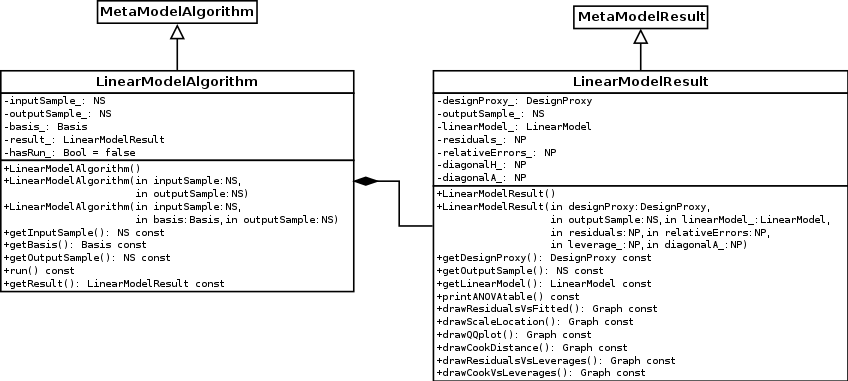
\includegraphics[scale=0.5]{LinearModelAlgorithm.png}
    \caption{LinearModelAlgorithm and LinearModelResult classes}\label{fig:archi:LinearModelAlgorithm}
  \end{center}
\end{figure}

\subsection{ANOVA table}

It is requested to give access to the following data:
\begin{itemize}
\item Linear model formula, in a textual form
\item Informations about residuals (minimum, maximum, median, mean, quantiles, standard deviation)
\item For each factor,
\begin{itemize}
\item its coefficient
\item its standard error
\item p-value for Student test
\item A visual symbol for significance test
\end{itemize}
\item Number of degrees of freedom
\item Coefficients $R^2$ and adjusted $R^2$
\item p-value of the Fisher test
\item normality tests on residuals (Kolmogorov-Smirnov, Anderson-Darling and $\chi^2$)
\end{itemize}

Note: Student test uses
\[
\frac{\hat{\beta}_i}{\sqrt{\frac{n}{n-p-1}\left[(X^T X)^{-1}\right]_{i,i}}}
\]

\subsection{Graphical diagnostics}

Several plots are provided by \texttt{LinearModelResult} class, see diagram class.
\begin{itemize}
\item \texttt{drawResidualsVsFitted} plots standardized residuals $\tilde{\epsilon}$ vs. fitted values, with
\[
\tilde{\epsilon}_i = \frac{\hat{\epsilon}_i}{\sqrt{\frac{n}{n-p-1}\hat{\sigma}^2 (1-H_{i,i})}}
\]
\item \texttt{drawQQPlot} plots $\sqrt{|\tilde{\epsilon}_i|}$ vs. theoretical quantiles.
\item \texttt{drawScaleLocation} plots $\sqrt{\tilde{\epsilon}_i}$ vs. fitted values.
\item \texttt{drawCookDistance} plots an histogram of Cook's distance
\[
D_i = \frac{\tilde{\epsilon}_i^2}{p} \left(\frac{H_{i,i}}{1-H_{i,i}}\right)
\]
\item \texttt{drawResidualsVsLeverages} plots standardized residuals $\tilde{\epsilon}$ vs leverages
\[
h_i = H_{i,i}
\]
Moreover, this plot also contains contour plot of function
\[
D(x,y) = \frac{y^2}{p}\left(\frac{x}{1-x}\right)
\]
for levels $0.5$ and $1$.
\item \texttt{drawCookVsLeverages} plots Cook's distance $\tilde{\epsilon}$ vs $\frac{h_i}{1-h_i}$.
\[
h_i = H_{i,i}
\]
Moreover, this plot also contains isolines of function
\[
\frac{py}{x}
\]
\end{itemize}

All these plots must display labels of some extremal points.  To this end, the following attributes
and methods will be added to \texttt{Cloud} and \texttt{BarPlot}:
\begin{verbatim}
   /** Setter for labels */
   Description getLabels() const;
   void setLabels(const Description & labels);
   /** Labels */
   Description labels_;
\end{verbatim}
The \texttt{labels} argument must have the same size as graph data, and only non-empty labels are
printed.
